\chapter{Dimensionering af stålprofiler}

Figur \ref{fig:hej} viser de nye byggefelter inden for henholdsvis delområde A og delområde B til Strøybergs Palæ (\citep{lokalplan}, s. 16). Denne rapport fokuserer på byggefeltet inden for delområde B, hvor ny bebyggelse, ifølge lokalplan 1-1-107, må opføres i 3 etager samt en tagetage og med en kælder maksimalt 2 m over terræn. Ved opførsel af ny bebyggelse i delområde B, skal to nuværende mindre bygninger fjernes. 

\begin{figure}[htbp]
	\centering
	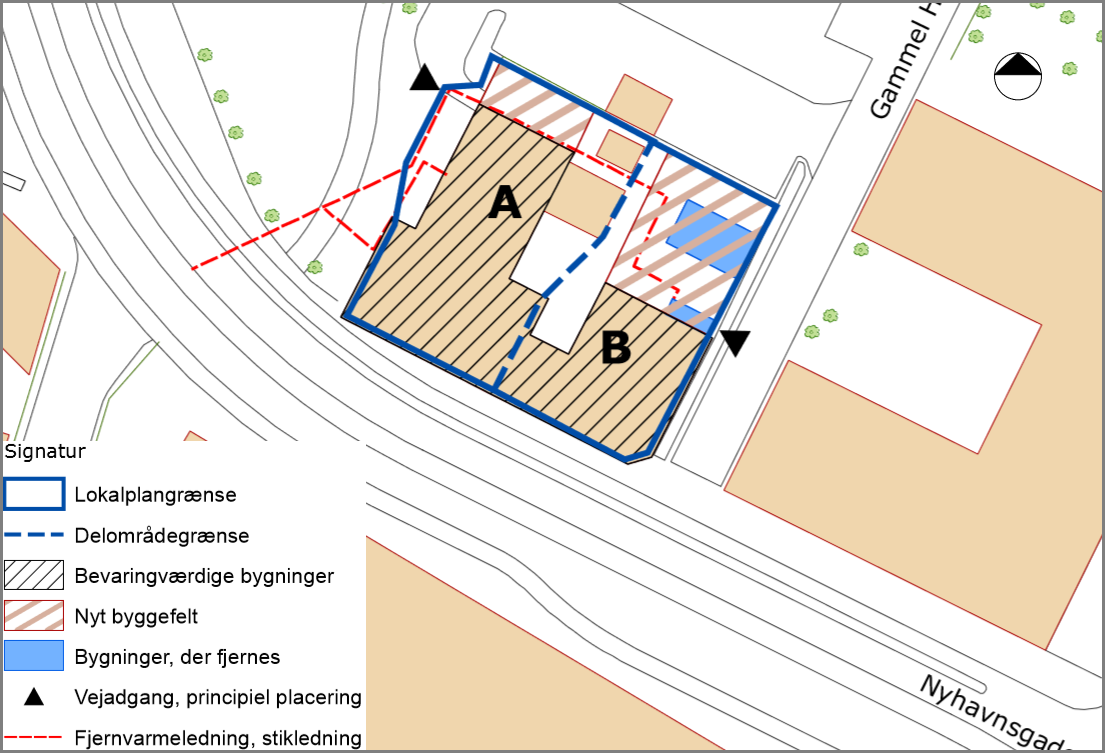
\includegraphics[width=0.8\textwidth]{billeder/signatur.png}
	\caption{Lokalplan 1-1-107, delområde A og B \citep[ bilag 2, s. 35]{lokalplan}}
	\label{fig:hej}
\end{figure}

Med udgangspunkt i lokalplan 1-1-107 har bygningen fået de størrelser og dimensioner, som ses på Figur \ref{fig:farvel}, som videre beregninger tager udgangspunkt i.
\newline \indent{     }  Tilbygningen bliver $12,\!5$ meter lang og 12 meter bred i henhold til den eksisterende bygningsbredde. Kælderen har en højde på i alt $3,\!25$ m, hvor $1,\!25$ m ligger over terræn. Stueetagen, 1. sal og 2. sal har hver især en højde på $4,\!9$ m og tagetagen har en højde på 3 meter med en hældning på $26,\!6$ grader. I alt er tilbygningen 19 m høj over terræn.

\begin{figure}[H]
	\centering
	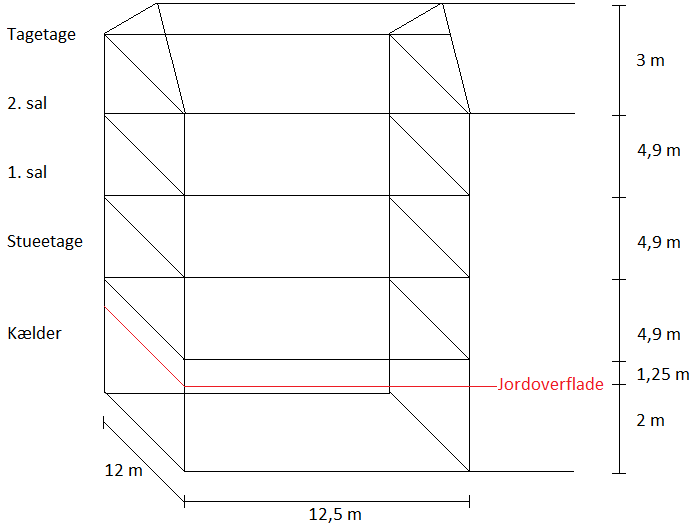
\includegraphics[width=0.8\textwidth]{billeder/tilbygning2.png}
	\caption{Tilbygningens dimensioner}
	\label{fig:farvel}
\end{figure}

For at kunne beregne de laster som påvirker tilbygningen, er der opstillet et statisk system som ses på Figur \ref{fig:system}. Systemet er opstillet som en bjælkekonstruktion. Som det ses på Figur \ref{fig:farvel} er der tre stålrammer; en i midten og en i hver af gavlene. I videre beregninger foretages der beregninger for rammen i midten.

\begin{figure}[H]
	\centering
	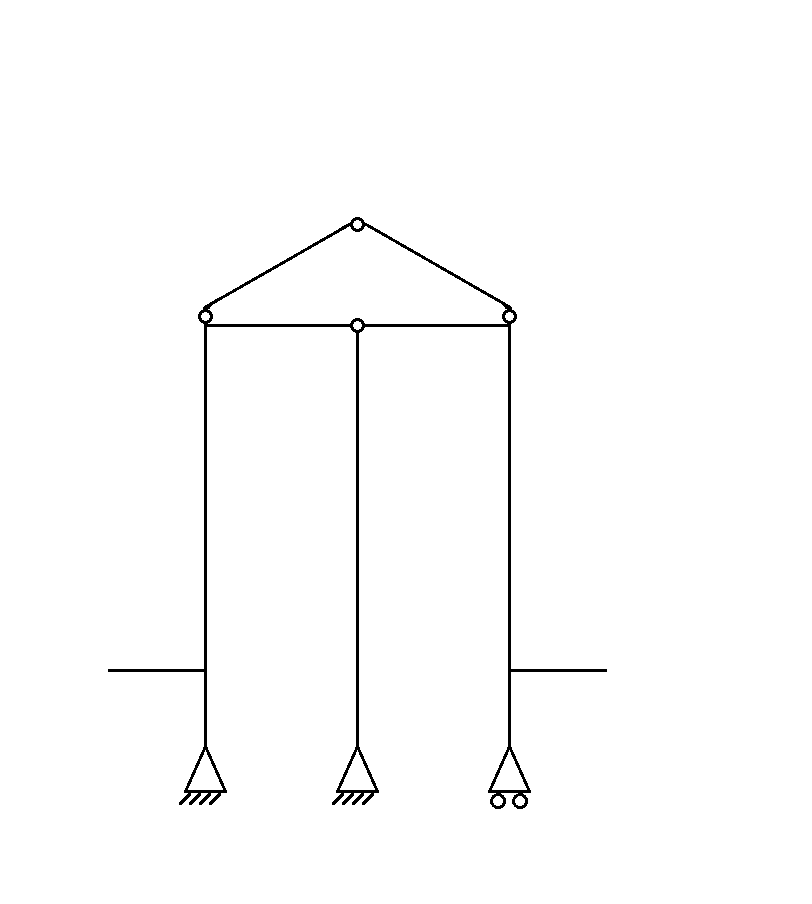
\includegraphics[width=0.4\textwidth]{billeder/del1statiskesystem.png}
	\caption{Statisk system}
	\label{fig:system}
\end{figure}

Etagedækkene vil virke som en belastning og ses ikke som en del af konstruktionen. Dette er muligt, da der opsættes en samling mellem etagedækkene og stålkonstruktion, som ses på Figur \ref{fig:etage}.

\begin{figure}[H]
	\centering
	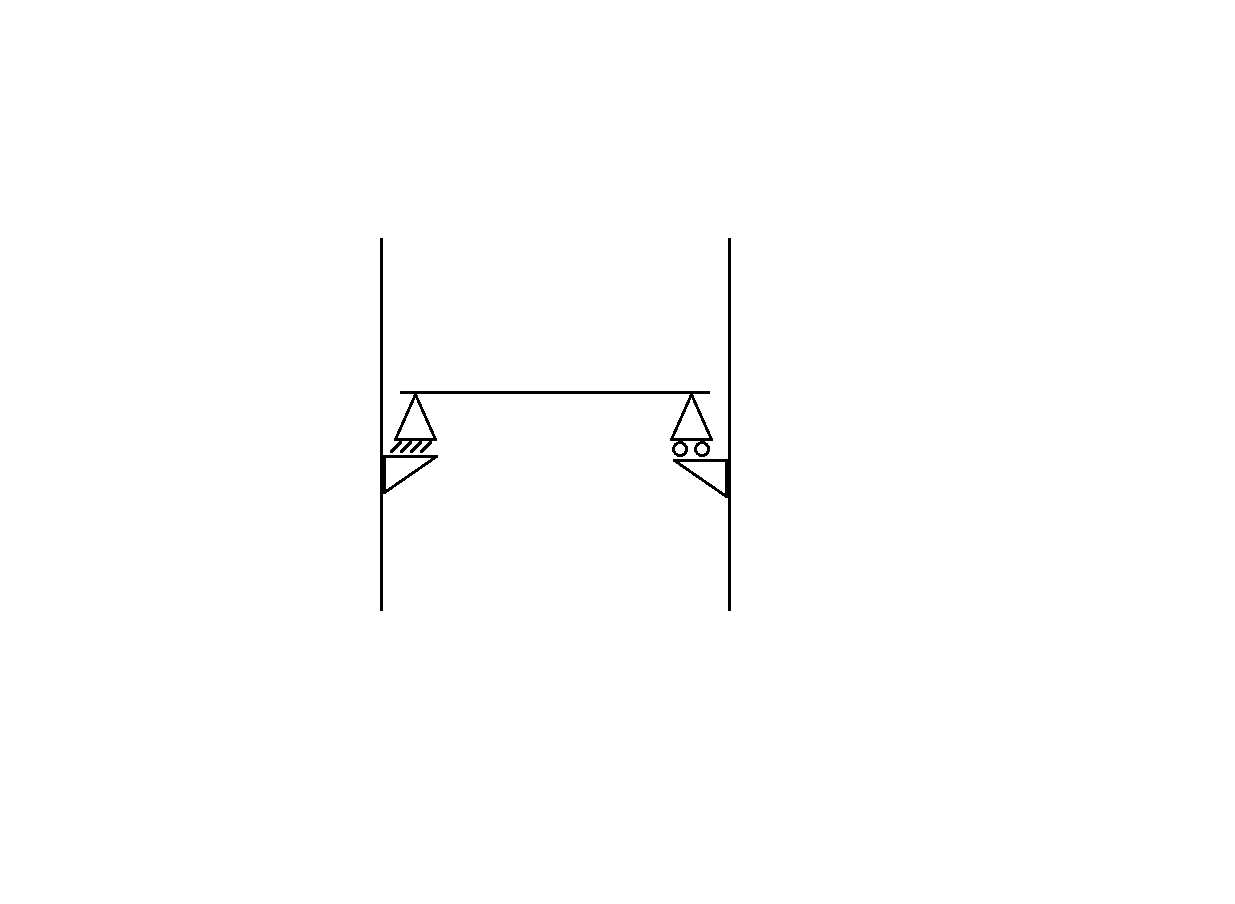
\includegraphics[width=0.2\textwidth]{billeder/etageovergang.png}
	\caption{Etageovergang på tilbygningen}
	\label{fig:etage}
\end{figure}

Ståltypen for det statiske system sættes til at være ståltype S235 med profilnummer 450 \citep{stabi}.

\section{Laster}
Tilbygningen til Strøybergs Palæ vil blive udsat for en række laster, både permanente- og variable laster. Disse vil blive beregnet i dette afsnit, så der kan opstilles lastkombinationer samt beregnes brudgrænse- og anvendelsesgrænsetilstande.

\subsection{Permanente laster}
De permanente laster, der beregnes for tilbygningen af Strøybergs Palæ, er egenlast og jordlast.

\subsubsection{Egenlast}
Når egenlasten skal bestemmes...

\textbf{Last fra tag}
\newline
Det antages, at taget er et mellemtungt sadeltag med teglsten, som har egenvægt $600 \frac{N}{m^2}$ \citep{tag}.
\newline
\newline
Tagets areal bestemmes ud fra Figur \ref{fig:tagetage}:
\begin{center}
	$A_{tag} = 6,\!7 m\cdot 12,\!5 m \cdot 2=167,\!500 m^2$
\end{center}

Arealet multipliceres med egenvægten for mellemtungt tag:
\begin{center}
	$p_{tag} = 167,\!500 m^2\cdot 600 \frac{N}{m^2}=100,\!500 kN$
\end{center}

\begin{figure}[H]
	\centering
	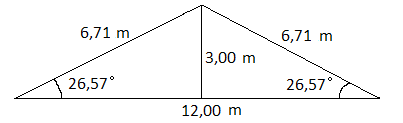
\includegraphics[width=0.7\textwidth]{billeder/Tagmedvinkel.png}
	\caption{Dimensioner for tagetagen}
	\label{fig:tagetage}
\end{figure}

Dermed er lasten fra taget $100,\!500 kN$, som vil blive brugt til videre beregninger.
\newline
\newline
\textbf{Last fra væg}
\newline
Facaderne antages at være ens samt indeholde lige mange vinduer og døre. Der antages at være 11 vinduer og én dør pr. facade \citep{gammellokalplan}, hvilket illustreres med mål på Figur \ref{fig:facade}.

\begin{figure}[H]
	\centering
	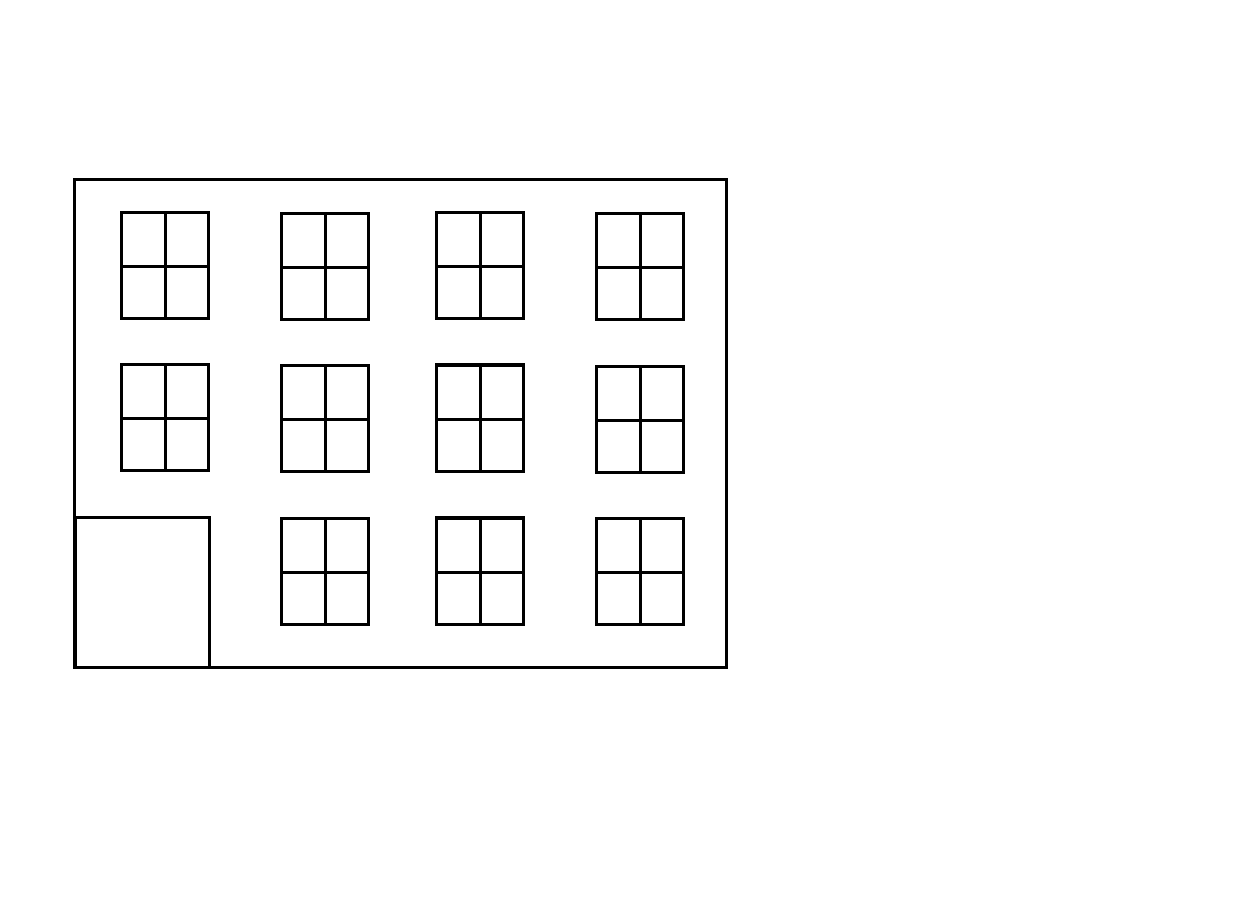
\includegraphics[width=0.8\textwidth]{billeder/facadenord.png}
	\caption{Facaden på øst- og vestsiden}
	\label{fig:facade}
\end{figure}

Til beregning af væggens egenlast skal der påregnes en indervæg og et isoleringslag. Ydervæggen ikke er en del af det statiske system og dermed ikke skal medregnes. Indervæggen bestemmes til at være mursten, mens isoleringen bestemmes til at være rockwool. Tykkelsen og densiteten for mursten og rockwool kan ses i Tabel \ref{tab:murogwool}.

\begin{table}
	\begin{center}
		\begin{tabular}{|c|c|c|}
			\hline
			& Densitet, d [$\frac{kg}{m^3}$] & Tykkelse, t [mm] \\ \hline
			Mursten  & 1500  & 130     \\ \hline
			Rockwool & 30 & 100              \\ \hline
		\end{tabular}
		\caption{Materialer og deres egenskaber for væg \citep{murstendensitet} \citep{indervaeg} \citep{densitet} \citep{isolering}}
		\label{tab:murogwool}
	\end{center}
\end{table}

Da den ene gavl ligger op ad den nuværende bygning, antages denne side ikke at belaste det statiske system. 
\newline \indent{     }  De 9 vinduer på gavlen, der ikke ligger op ad den nuværende bygning, er identiske med dem på facaden, som kan ses på Figur \ref{fig:gavl}. Indervæg og isolering for gavlen er ligeledes identisk med facadens.
\newline \indent{     }  Når arealet af facaderne beregnes trækkes arealet af vinduerne samt døren fra, da disse antages at belaste ydermuren.

\begin{figure}[H]
	\centering
	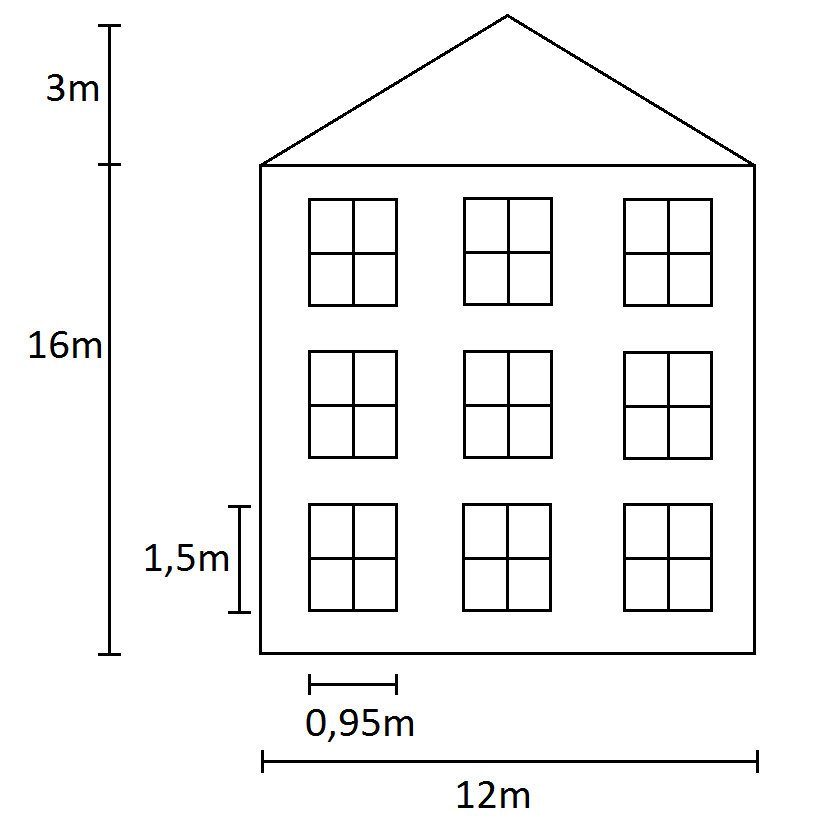
\includegraphics[width=0.6\textwidth]{billeder/facadevestellerost.png}
	\caption{Dimensioner for tagetagen}
	\label{fig:gavl}
\end{figure}

Arealerne og lasten for facaderne og gavlen kan ses i Tabel \ref{tab:arealoglast}, hvor lasten bestemmes ud fra formlen:
\begin{center}
	$p = g A \sum dt$
\end{center}

\begin{table}
	\begin{center}
		\begin{tabular}{|c|c|c|}
			\hline
			& Areal, A [$m^2$]   & Last, p [kN]    \\ \hline
			Facade, vest & 181,18 & 352,27 \\ \hline
			Facade, øst  & 181,18 & 352,27 \\ \hline
			Gavl, nord   & 197,18 & 383,38 \\ \hline
		\end{tabular}
		\caption{Areal og last for væg}
		\label{tab:arealoglast}
	\end{center}
\end{table}

\textbf{Last fra gulv}
\newline
Det antages at bygnings etager kun består af gulv, dvs. ingen skillevægge, trapper m.m. Derfor er den samlede mængde gulv pr. etage: 

\begin{center}
$A_{etage} = 12,\!50 m\cdot 12,\!00 m = 150,\!00 m^2$
\end{center}

Fire ud af fem etager består af bærende gulv. Kælderetagen ligger på fundamentet og regnes derfor ikke som et bærende gulv. 
\newline \indent{     }  Et bærende gulv antages at bestå af et armeret betondæk nederst, der oftest er mellem 80 mm og 200 mm tyk. Det bestemmes, at den er 120 mm tyk, hvorpå der ligger bjælker. Bjælkernes opgave er at lede og overføre lasterne ud i understøtning. Derefter vil ligge et undergulv, mellemgulv og til sidst selve gulvbelægningen, og mellem betondækket og undergulvet lægges isoleringen \citep{Gulvopbygning}. Densiteten og tykkelsen af gulvlagene kan ses i Tabel \ref{tab:densi}.

\begin{table}
	\begin{center}
		\begin{tabular}{|c|c|c|}
			\hline
			& Densitet [$\frac{kg}{m^3}$] & Tykkelse [mm] \\ \hline
			Beton    & 2400     & 120      \\ \hline
			Rockwool & 30       & 140      \\ \hline
			Linoleum & 2,9      & 383,38  \\ \hline
		\end{tabular}
		\caption{Materialer og deres egenskaber for gulv}
		\label{tab:densi}
	\end{center}
\end{table}

Der er behov for bjælker, som hver er $6,\!25$ m lang, da de er halvdelen af tilbygningens længde, $140,\!00$ mm høj og $140,\!00$ mm bred \citep{granse}. Disse anlægges langs med tilbygningen. For at bestemme hvor mange bjælker, der er behov for, divideres længden af tilbygningen med 400 mm, da der skal være 400 mm imellem hver bjælke \citep{Gulvopbygning}. 

\begin{center}
	$\frac{12,\!50 m}{0,\!40 m}=31,\!25$ bjælker
\end{center} 

Da der ikke kan optræde $31,\!25$ bjælker rundes der op til 32 bjælker.
\newline
\newline
Rumfanget af de 32 bjælker med længden $12,\!5$ m multipliceres med bjælkens densitet for tørrumvægt af træ \citep{torrumvagt}, som er $510 \frac{kg}{m^3}$, hvorefter denne værdi multipliceres med tyngdeaccelerationen og multipliceres med 4, da der er fire etager foruden kælderen. Herved findes lasten for bjælkerne: 
\begin{center}
	$p_{bjælker} = 7,\!84 m^3\cdot 510 \frac{kg}{m^3}\cdot 9,\!82 \frac{m}{s^2}\cdot 4 = 157,\!06 kN$
\end{center}

Beregning af volumen og last for beton, rockwool og linoleum beregnes på samme måde som for bjælkerne, dog skal bjælkernes volumen trækkes fra ved beregning af værdierne for rockwool. Resultaterne kan ses i Tabel \ref{tab:gulv}.

\begin{table}
	\begin{center}
		\begin{tabular}{|c|c|c|}
			\hline
			& Volume [$m^3$] & Last [kN] \\ \hline
			Bjælker	 & 31,36 & 157,06	\\ \hline
			Beton    & 72,00 & 1693,44     \\ \hline
			Rockwool & 52,64 & 15,51     \\ \hline
			Linoleum & 1,50 & 0,04     \\ \hline
		\end{tabular}
		\caption{Samlet volumen og last for gulvelementerne}
		\label{tab:gulv}
	\end{center}
\end{table}

\textbf{Samlet egenlast eksklusiv tag og stålsystem}
\newline
De tidligere beregnede værdier adderes; 
\begin{center}
	$346,\!932 kN + 346,\!932 kN + 5,\!337 kN + 5,\!337 kN + 377,\!509 kN + 5,\!809 kN + 1693,\!440 kN + 157,\!057 kN + 15,\!508 kN + 0,\!043 kN = 2953,\!904 kN$
\end{center}
Den samlede egenlast deles med 2, da midterrammen optager halvdelen af den beregnede last. 
\begin{center}
	$\frac{2953,904 kN}{2} =  1476,\!952 kN$
\end{center}
Den midterste stang optager $\frac{1}{2}$ af egenlasten, mens de to yderste stænger hver optager $\frac{1}{4}$, derfor divideres nu med 4.

\begin{center}
	$\frac{1476,952 kN}{4} =  369,\!24 kN$
\end{center}

Denne last laves nu om til en linjelast ned langs stængerne, og derfor deles med 18m:
 
\begin{center}
	$\frac{369,24 kN}{18m} =  20,\!51 \frac{kN}{m}$
\end{center} 

\textbf{Egenlast af stålsystemet}
\newline
Egenlast stål i tagsystemet:
\newline
Densiteten for den anvendte ståltype S235 med profil nr. 450 har densiteten $g=115\frac{kg}{m}$ \citep{stabi}. Dette skal ganges med højden af sadeltaget, som er $6,\!7m$ og omregnes efterfølgende til KiloNewton.  
\begin{center}
	$115\frac{kg}{m}\cdot 6,\!7m = 771,\! 42 kg$
\end{center}

\begin{center}
	$771,\! 42kg\cdot 9,\! 82\frac{m}{s^2} = 7,\! 5753444 kN$
\end{center}

Denne værdi skal ganges med to, da der går to stålstænger op ved taget:

\begin{center}
$7,\! 58kN \cdot 2 = 15,\! 1506888 kN$
\end{center}

Stålsystem eksklusiv tag:
\newline
Stålstyrken antages igen at være S235, som har densiteten $g=115\frac{kg}{m}$ \citep{stabi}. For at finde kraften af en enkelt lodret stang multipliceres denne med højden af bygningen, som er 18 m, inklusiv kælderen.
\begin{center}
	$115\frac{kg}{m}\cdot 18m = 2070 kg$
\end{center}

\begin{center}
	$2070 kg \cdot 9,\!82\frac{m}{s^2} = 20,\! 33 kN$
\end{center}

Dette skal omregnes til at blive en linjelast og der divideres derfor med højden igen:

\begin{center}
$\frac{20,\! 33 kN}{18m} = 1,\! 13\frac{kN}{m}$
\end{center}

Det samme skal gøres for at finde kraften for en vandret stang, og densiteten skal her ganges med længden af den vandrette bjælke, som er 6 m.
\begin{center}
	$115\frac{kg}{m}\cdot 6m = 690 kg$
\end{center}

\begin{center}
	$690 kg \cdot 9,\!82\frac{m}{s^2} = 6,\!78  kN$
\end{center}

Dette skal omregnes til at blive en linjelast og der divideres derfor med længden af den vandrette stang:
$\frac{6,\! 78 kN}{6m} = 1,\! 13\frac{kN}{m}$
\newline
\newline
\textbf{Opsamling}
\newline
Nu er alle karakteristiske egenlaster fra taget, etagedækkene samt egenlasten fra bjælkesystemet bestemt. Disse placeres nu i det statiske sytem vidst på Figur \ref{fig:m} og \ref{fig:n}.

\begin{figure}[htbp]\centering
	\begin{minipage}[b]{0.48\textwidth}\centering
		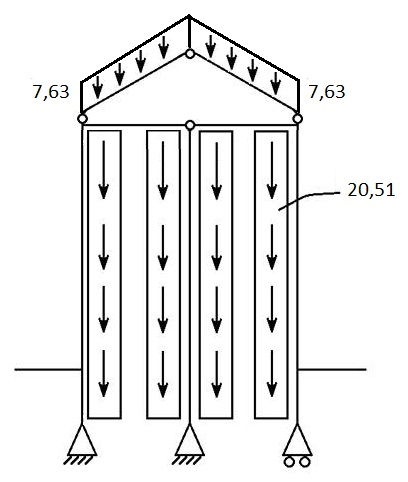
\includegraphics[width=0.80\textwidth]{billeder/egenlastetage.png} %Venstre billede
	\end{minipage}\hfill
	\begin{minipage}[b]{0.48\textwidth}\centering
		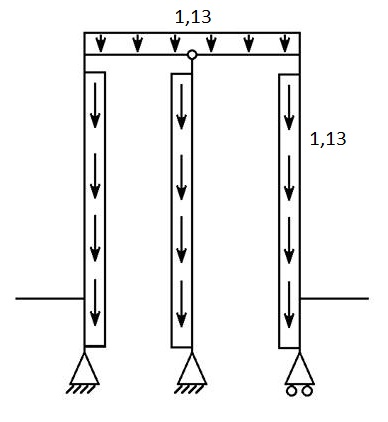
\includegraphics[width=0.8\textwidth]{billeder/egenlaststaal.png} %Højre billede
	\end{minipage}\\ %Captions and labels
	\begin{minipage}[t]{0.48\textwidth}
		\caption{Egenlast fra etagedæk angivet i $\frac{kN}{m}$} %Venstre caption og label
		\label{fig:m}
	\end{minipage}\hfill
	\begin{minipage}[t]{0.48\textwidth}
		\caption{Egenlast fra stålsystemet angivet i $\frac{kN}{m}$} %Højre caption og label
		\label{fig:n}
	\end{minipage}
\end{figure}

\subsubsection{Jordlast}
Idet tilbygningen har en kælder, der går 2 m under jorden, bliver den påvirket med en jordlast. Jordlasten virker på konstruktionen fra jordoverfladen og nedefter og virker liniært afhængigt af dybden.
\newline
\newline
Jordlasten beregnes gennem formlen:
\begin{center}
	$\sigma_x = k_0 \sigma_z$
\end{center}

\begin{itemize}
	\item[-] $k_0$: hviletrykskoefficienten, som er givet ved $k_0=1-sin(\varphi)$, hvor $\varphi$ er friktionsvinklen. Friktionsvinklen er bestemt igennem fire forsøg, som ses under Afsnit (!!!!!!)
	\item[-] $\sigma_z$: den lodrette fladelast i dybden z givet ved $\sigma_z = z\gamma$, hvor z er dybden og $\gamma$ er rumvægten $[\frac{kN}{m^3}]$
\end{itemize}

Hviletrykskoefficenten, $k_0$ bestemmes:
\begin{center}
	$k_0 = 1 - sin(32,\!33) = 0,\!47$
\end{center}

Rumvægten slås op til $20 \frac{kN}{m^3}$ \citep[ s. 386]{stabi} og den lodrette fladelast, $\sigma_z$, bestemmes:
\begin{center}
	$\sigma_z = z\cdot 20 \frac{kN}{m^3}$
\end{center}

Nu er hviletrykskoefficienten og fladlasten bestemt, og det betyder, at jordlasten $\sigma_x$, i dybderne z for 0 m og 2 m bestemmes:
\begin{center}
	$\sigma_x = 0,\!47\cdot 0 m\cdot 20 \frac{kN}{m^3} = 0 \frac{kN}{m^2}$
\end{center}

\begin{center}
	$\sigma_x = 0,\!47\cdot 2 m\cdot 20 \frac{kN}{m^3} = 18,\!61 \frac{kN}{m^2}$
\end{center}

I og med jordlasten ved 0 m er $0 \frac{kN}{m^2}$, vil den også optræde som en linjelast med værdien $0 \frac{kN}{m}$. Dermed beregnes linjelasten for dybden 2 m, ved at multiplicere med længden, som den virker over, hvilken er 6,25 m:
\begin{center}
	$\sigma_{x,linje} = 18,\!61 \frac{kN}{m^2}\cdot 6,\!25 m = 116,\!32 \frac{kN}{m}$
\end{center}

Dermed er jordlasten, som linjelast, i dybderne som ses på Tabel \ref{tab:jord}.
\begin{table}[htb]
	\begin{center}
		\begin{tabular}{ |c|c|c| } 
		\hline
		Dybde [m] & 0 & 2 \\ \hline
		Jordlast $[\frac{kN}{m}]$ & 0 & 116,32 \\ \hline
		\end{tabular}
		\caption{Værdier for jordlasten}
		\label{tab:jord}
	\end{center}
\end{table}

For at finde den jordlast der virker over x-antal meter under jorden, opstilles følgende ligning:

\begin{center}
	$w = \frac{1}{2} \cdot x \cdot p$
\end{center}

\begin{itemize}
	\item[-] x: længden, som kraften virker over
	\item[-] p: den største kraft
\end{itemize}

Hermed fås ligningen: 
\begin{center}
	$w = \frac{1}{2} 116,\!32 \frac{kN}{m} x = 58,\!16x$
\end{center}

Den jordlast der virker på det statiske system er illustreret på Figur \ref{fig:jordlast}.

\begin{figure}[H]
	\centering
	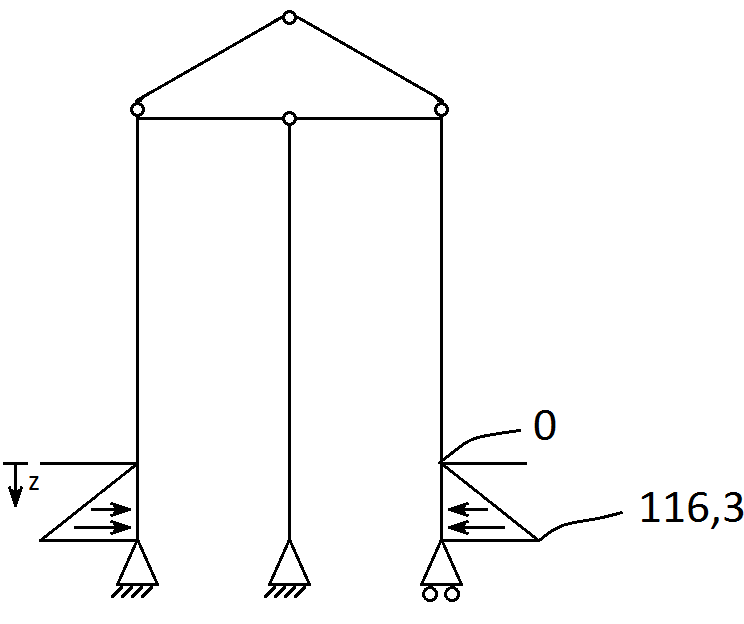
\includegraphics[width=0.5\textwidth]{billeder/jordlast.png}
	\caption{Jordlast på det statiske system angivet i $\frac{kN}{m}$}
	\label{fig:jordlast}
\end{figure}


\subsection{Variable laster}
Af variable laster optræder snelast, vindlast og nyttelast på bygningen. Disse udregnes efter Dansk Standard Eurocode 1991.

\subsubsection{Snelast}
Til at beregne den karakteristiske snelast anvendes følgende formel:
\begin{center}
	$s=\mu_iC_eC_ts_k$
\end{center}
\begin{itemize}
	\item[-] $\mu_i$: formfaktoren for snelasten, som sættes til 0.8 \citep[ tabel 5.2 kapitel 5.3]{EU91}
	\item[-] $C_e$: eksponeringsfaktoren
	\item[-] $C_t$: termisk faktor, som sættes til $1,\!0$ \citep[ kapitel 5.2]{EU91}
	\item[-] $s_k$: karakteristisk terrænværdi, som sættes til $1 \frac{kN}{m^2}$ \citep[ kapitel 4.1]{EU91}
\end{itemize}

Eksponeringsfaktoren, $C_e$, bestemmes ved:
\begin{center}
$C_e=C_{top}C_s$
\end{center}
\begin{itemize}
	\item[-] $C_{top}$: topografi faktor, som sættes til $1,\!0$ \citep[ tabel 5.1 kapitel 5.2]{EU91}
	\item[-] $C_s$: størrelse faktor, som sættes til $1,\!0$ \citep[ kapitel 5.2]{EU91}
\end{itemize}
Eksponeringsfaktoren kan nu bestemmes til:
\begin{center}
$C_e=1,\!0\cdot 1,\!0=1,\!0$
\end{center}
Strøybergs Palæ har et sadeltag, og dermed skal der tages højde for fire lasttilfælde, som ses på Figur \ref{fig:sne}. Derudover multipliceres snetilfældets værdi med 6,25 m, som er halvdelen af tilbygningens længde, hvilket gøres, da det statiske system er opdelt i tre rammer, for at få værdien ud i $\frac{kN}{m}$.

\begin{figure}[htbp]
	\centering
	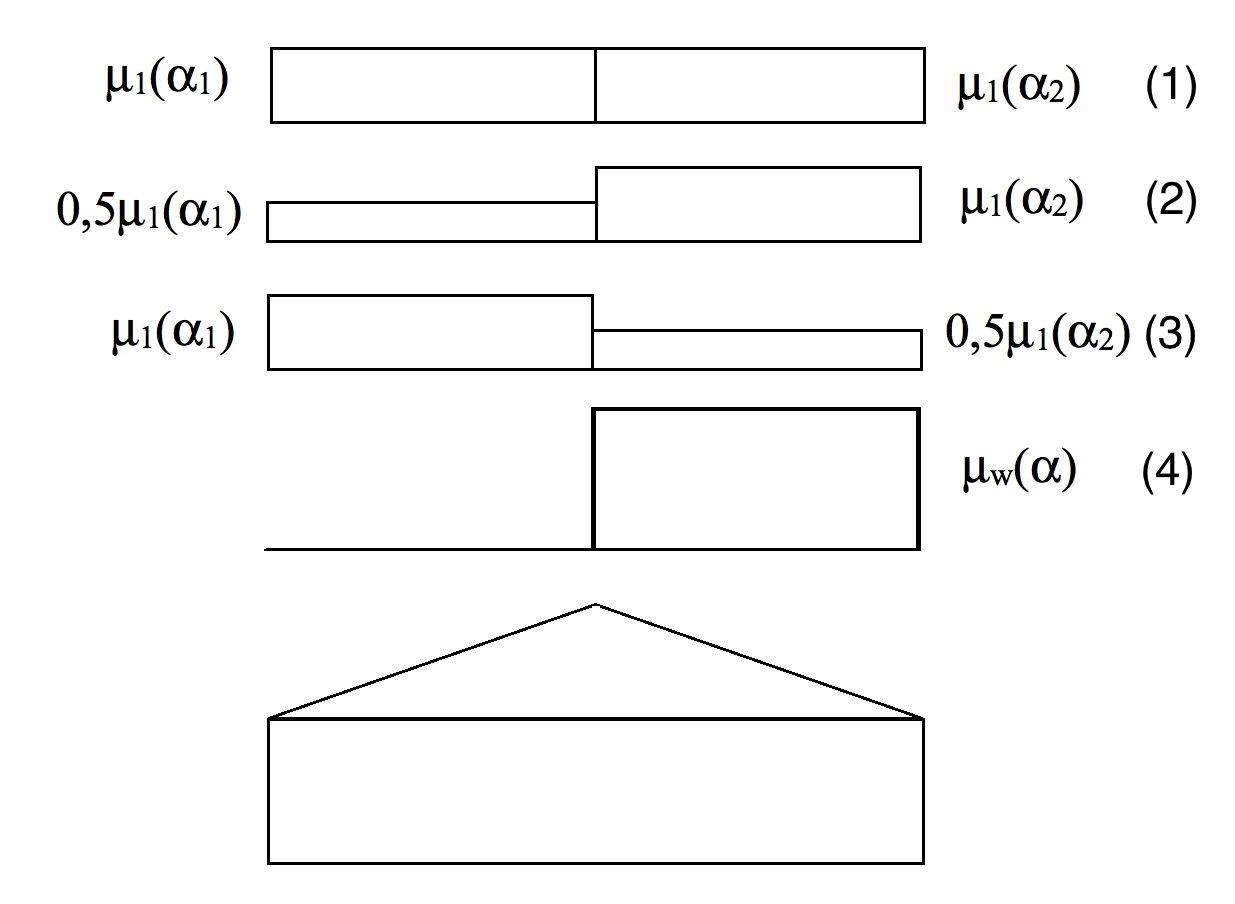
\includegraphics[width=0.6\textwidth]{billeder/snelasttilfaelde.png}
	\caption{Fordeling af sne i de fire tilfælde \citep[ kapitel 5.3.3]{EU91}}
	\label{fig:sne}
\end{figure}

\underline{Snetilfælde 1}
\begin{center}
$s_1=0,\!8\cdot 1.0\cdot 1,\!0\cdot 1 \frac{kN}{m^2}\cdot 6,\!25 m=5,\!0 \frac{kN}{m}$
\end{center}
\underline{Snetilfælde 2 og 3}
\begin{center}
$s_2=\frac{1}{2}\cdot 0,\!8\cdot 1,\!0\cdot 1,\!0\cdot 1 \frac{kN}{m^2}\cdot 6,\!25 m=2,\!5 \frac{kN}{m}$
\end{center}
\underline{Snetilfælde 4}
\newline
\newline
Snetilfælde 4 er ophobning, og dermed anvendes en anden formfaktor.
\begin{center}
	$s_4=\mu_wC_eC_ts_k$
\end{center}
\begin{itemize}
	\item[-] $\mu_w$: formfaktoren, som sættes til $1,\!2$ eftersom $\alpha$ er $26,\!56^{\circ}$ \citep[ kapitel 5.3.3]{EU91}
\end{itemize}
Den karakteristiske snelast for lasttilfælde 4 kan nu bestemmes til:
\begin{center}
	$s_4=1,\!2\cdot 1,\!0\cdot 1,\!0\cdot 1 \frac{kN}{m^2}\cdot 6,\!25 m = 7,\!5 \frac{kN}{m}$
\end{center}
Til videre beregning har projektgruppen valgt at anvende snetilfælde 1, som er illustreret på Figur \ref{fig:sne}. I praksis burde der laves beregninger med samtlige snetilfælde.

\begin{figure}[H]
	\centering
	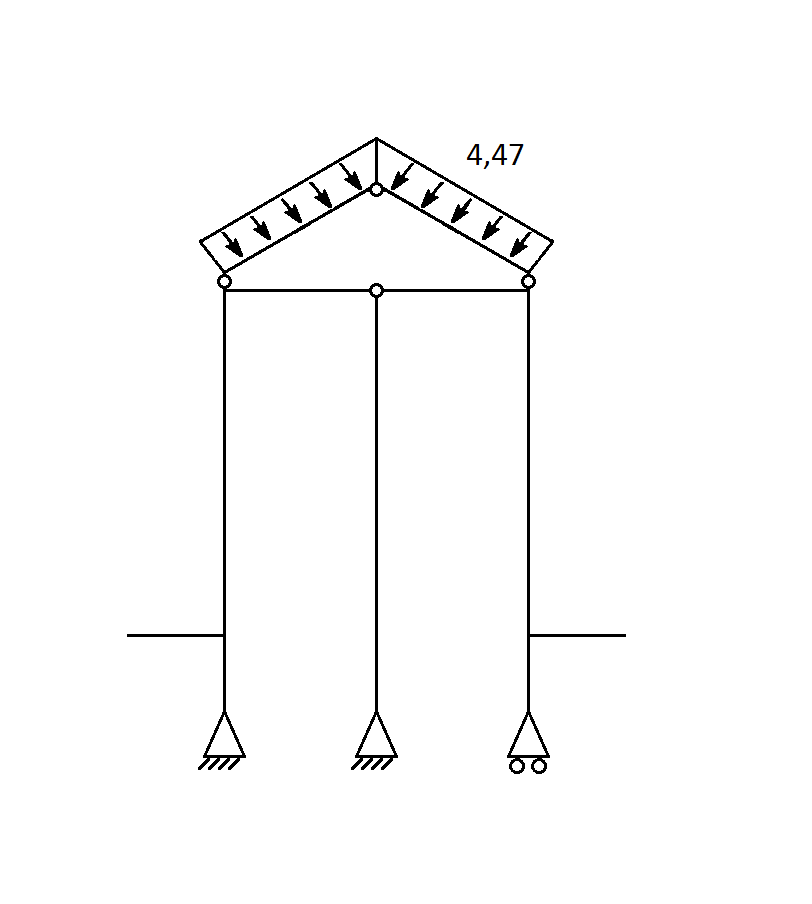
\includegraphics[width=0.3\textwidth]{billeder/snelast.png}
	\caption{Snelast på det statiske system angivet i $\frac{kN}{m}$}
	\label{fig:snelast}
\end{figure}

\subsubsection{Vindlast}
For vindlasten regnes der en nettovindlast, hvilken regnes som summen af den udvendige og den indvendige vindlast.
\newline \indent{     }  For Strøybergs Palæ regnes der en nettovindlast for taget og for facaderne på bygningen, hvilket gøres for tre vindretninger, nord, øst og vest, da sydsiden af tilbygningen kommer i forlængelse af den allerede eksisterende bygning, og derfor formodes denne vindlast ikke at have en særlig betydning for tilbygningen.
\newline
\newline
Til at bestemme vindlasten på tilbygningens udvendige sider anvendes følgende formel:	
\begin{center} 
	$w_e=q_p(z_e)c_{pe}$
\end{center}
\begin{itemize}
	\item[-] $q_p$: peakhastighedstrykket
	\item[-] $z_e$: referencehøjden for det udvendige vindtryk, som er 19 m for taget og 16 m for facaderne
	\item[-] $c_{pe}$: formfaktoren for det udvendige vindtryk
\end{itemize}

Til at bestemme vindlasten på tilbygningens indvendige sider anvendes følgende formel:
\begin{center} 
	$w_i=q_p(z_i)c_{pi}$
\end{center}
\begin{itemize}
	\item[-] $q_p$: peakhastighedstrykket
	\item[-] $z_i$: referencehøjden for det indvendige vindtryk, som sættes lig det udvendige for hhv. tag og facader $z_e$ \citep[ kapitel 7.2.9]{EU91}
	\item[-] $c_{pi}$: formfaktoren for det indvendige vindtryk
\end{itemize}

I Bilag A ses et beregningseksempel på bestemmelse af peakhastighedstrykket, $q_p$, og i Tabel \ref{tab:peak} ses værdierne for peakhastighedstrykket for alle tre vindretninger ved højderne 16 m og 19 m.
\begin{table}[htb]
\begin{center}
	\begin{tabular}{ |c|c|c| } 
		\hline
		Vindretning/Højden & $q_p [\frac{kN}{m^2}]$ ved 16 m & $q_p [\frac{kN}{m^2}]$ ved 19 m \\	\hline
		Vest & 0,536 & 0,579 \\		\hline
		Øst & 0,428 & 0,463 \\	\hline 
		Nord & 0,428 & 0,463 \\ 	\hline
	\end{tabular}
		\caption{Værdier for $q_p [\frac{kN}{m^2}]$}
		\label{tab:peak}
\end{center}
\end{table}

Peakhastighedstrykket skal nu anvendes, for at bestemme vindlasten på taget fra de tre vindretninger.
\newline
\newline
\textbf{Vindtryk på tag}
\newline
Først bestemmes de karakteristiske vindlaster ved at opstille en række vindtilfælde for henholdsvis tryk og sug. Tryk regnes altid positiv, da denne virker mod taget, og sug regnes altid negativ, da denne virker væk fra taget.
\newline
\newline
Da tilbygningen til Strøybergs Palæ får et sadeltag, anbefales det at dele taget ind i zoner efter Eurodecode 1991. Bygningen tegnes i fuld størrelse, hvor længden \textit{e} er 25 m, og derfor er den nuværende bygning også medregnet i målene. For vindretningen $\theta = 0^{\circ}$ (gælder for vindretning fra vest og fra øst) skal bygningen deles ind som vist på Figur \ref{fig:opdeling}.  

\begin{figure}[htbp]
	\centering
	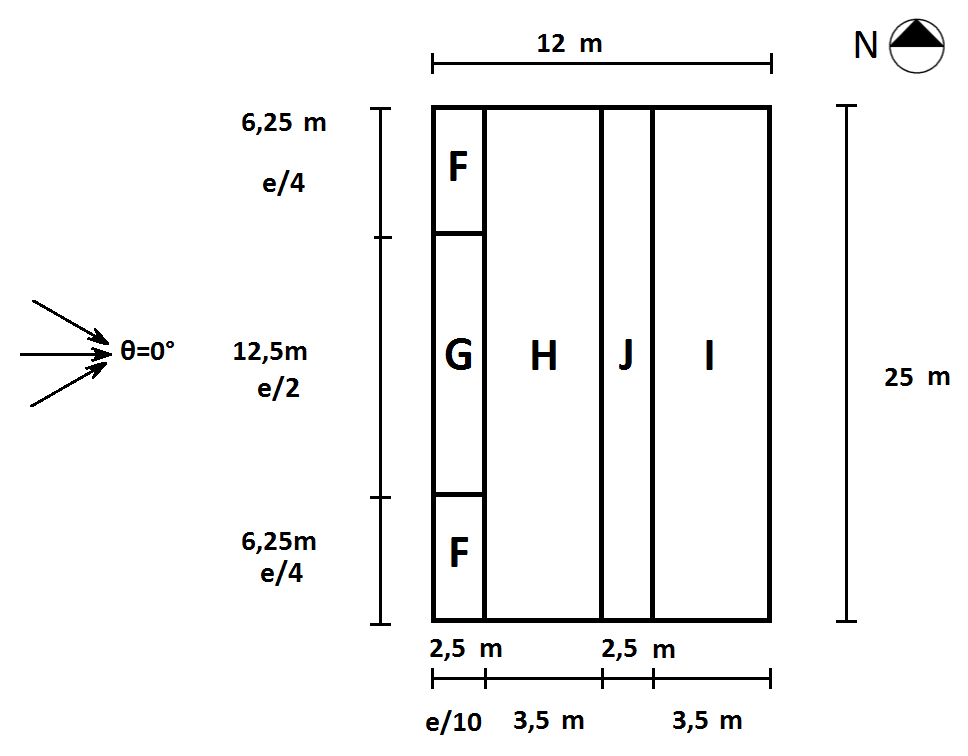
\includegraphics[width=0.8\textwidth]{billeder/opdeling.png}
	\caption{Opdeling af bygning, for vindretning fra øst og vest \citep[ kapitel 7.2.5]{EU91}}
	\label{fig:opdeling}
\end{figure}

Formfaktorerne, $c_{pe}$, for tagets zoner bestemmes ud fra Eurocode 1991. Her anvendes taghældningen på $\alpha = 26,\!56^{\circ}$, og der laves derfor lineær regression mellem $c_{pe}$ værdierne for vinklerne 15 og 30 grader, efter anbefaling af Eurocode 1991 \citep[ tabel 7.4a kapitel 7.2.5]{EU91}. For $\theta = 0^{\circ}$ skifter trykket hurtigt mellem positive og negative værdier i vindsiden, ved en taghældning mellem $\alpha = -5^{\circ} til + 45^{\circ}$, og derfor skal der regnes for både positive og negative formfaktorværdier. 
\newline \indent{     }  Nedenfor er et beregningseksempel for beregning af formfaktoren.
\newline
\newline
\underline{Zone F for vind fra vest}
\newline
Ud fra Eurocode 1991 \citep[ tabel 7.4a kapitel 7.2.5]{EU91} er de negative værdier for zone F: $-0,\!9$ og $-0,\!5$. Her ud fra laves lineær regression, og $c_{pe,10,neg}$ bestemmes:
\begin{center}
	$f(\alpha)=0,\!0267\alpha - 1,\!3 \to c_{pe,10,neg}=-0,\!592$
\end{center}
De positive værdier for zone F er: $0,\!2$ og $0,\!7$. Her ud fra fås ligningen, og $c_{pe,10,pos}$ bestemmes:
\begin{center}
	$f(\alpha)=0,\!0333\alpha - 0,\!3 \to c_{pe,10,pos}=0,\!585$
\end{center}

De beregnede værdier for formfaktorerne ses i Tabellerne; \ref{tab:cc} og \ref{tab:kk}. 
\newline
\newline
De udvendige vindtryk beregnes ved formlen, som tidligere vist:
\begin{center} 
	$w_e=q_p(z_e)c_{pe}$
\end{center}
Disse værdier findes alle i Bilag - HUSK REFERENCE! 
\newline
\newline
De indvendige vindtryk skal nu bestemmes, da de virker på samme tid som de udvendige vindtryk.
\newline
\newline
Der findes to måder til bestemmelse af formfaktoren, $c_{pi}$, for indvendig vind. I dette projekt anvendes den forsimplede metode, hvor $c_{pi}$ regnes til at være den mindst gunstige af + 0,2 og - 0,3 \citep[Kapitel 7]{EU91}. Værdierne for formfaktoren ses i Tabellerne \ref{tab:cc} og \ref{tab:kk}.
\newline
\newline
Herefter kan de indvendige vindtryk beregnes ved formlen, som tidligere vist:
\begin{center} 
	$w_e=q_p(z_e)c_{pi}$
\end{center}

\begin{table}[htb]
	\begin{center}
		\begin{tabular}{ |c|c|c|c|c| } 
			\hline
			Zone/Formfaktor & \multicolumn{2}{l|}{$c_{pe,10 udvendig}$} & \multicolumn{2}{l|}{$c_{pe,10 indvendig}$} \\	\hline
			& Positiv & Negativ & Positiv & Negativ \\ \hline
			F & 0,585 & -0,592 & 0,200 & -0,300 \\	\hline
			G & 0,585 & -0,569 & 0,200 & -0,300 \\	\hline 
			H & 0,354 & -0,223 & 0,200 & -0,300 \\ 	\hline
			I & 0 & -0,400 & 0,200 & -0,300 \\	\hline
			J & 0 & -0,615 & 0,200 & -0,300 \\	\hline
		\end{tabular}
		\caption{Værdier for $c_{pe,10}$ på udvendige og indvendige tagoverflader for vind fra vest og øst, vindretning $0^{\circ} = 180^{\circ}$ på taget}
		\label{tab:cc}
	\end{center}
\end{table}

\begin{table}[htb]
	\begin{center}
		\begin{tabular}{ |c|c|c|c| } 
			\hline
			Zone/Formfaktor & $c_{pe,10 udvendig}$ & \multicolumn{2}{l|}{$c_{pe,10 indvendig}$} \\	\hline
			& Negativ & Positiv & Negativ \\ \hline
			F & -1,146 & 0,200 & -0,300 \\	\hline
			G & -1,377 & 0,200 & -0,300 \\	\hline 
			H & -0,754 & 0,200 & -0,300 \\ 	\hline
			I & -0,500 & 0,200 & -0,300 \\	\hline
		\end{tabular}
		\caption{Værdier for $c_{pe,10}$ på udvendige og indvendige tagoverflader for vind fra nord, vindretning $90^{\circ}$ på taget}
		\label{tab:kk}
	\end{center}
\end{table}

For at bestemme nettovindtrykket skal der opstilles en række tilfælde for, hvordan det udvendige vindtryk og det indvendige vindtryk kan optræde.  
\newline
\newline
Der opstilles fire vindkombinationer for hver vindretning:
\begin{enumerate}
	\item Tryk udvendigt på FGH + sug for JI og invendigt sug
	\item Tryk udvendigt på FGH + sug for JI og invendigt tryk
	\item Sug udvendigt for FGH + tryk på JI og invendigt sug
	\item Sug udvendigt for FGH + tryk på JI og invendigt tryk
\end{enumerate}

Nedenfor laves et beregningseksempel med vind fra vest med vindkombination 1 for zone F. De resterende værdier kan ses i Tabel \ref{tab:bb}.
\newline
\newline
Enheden skal være $[\frac{kN}{m}]$, og derfor multipliceres med længden mellem hver af vores stænger, som er 6,25 m. Se Figur \ref{fig:farvel}.

\begin{center} 
	$w_F=(w_{e,F}-w_{i,F})\cdot 6,\!25 m$
\end{center}

\begin{itemize}
	\item[-] $w_{e,F}$: udvendigt vindtryk for zone F = $0,\!339 \frac{kN}{m^2}$
	\item[-] $w_{i,F}$: indvendigt vindtryk for zone F = $-0,\!174 \frac{kN}{m^2}$
\end{itemize}

\begin{center} 
	$w_F=(w_{e,F}-w_{i,F})\cdot 6,\!25 m = (0,\!339 \frac{kN}{m^2} - (-0,\!174 \frac{kN}{m^2})\cdot 6,\!25 m = 3,\!203 \frac{kN}{m}$
\end{center}

For alle vindretningerne anvendes vindkombination 1 til videre beregning, og disse laster ses i Tabel \ref{tab:bb}. 

\begin{table}[htb]
	\begin{center}
		\begin{tabular}{ |c|c|c|c| } 
			\hline
			Zone/Vindretning, w $[\frac{kN}{m}]$ & Vest & Øst & Nord \\	\hline
			F & 3,203 & 2,563 & -2,445 \\	\hline
			G & 3,203 & 2,563 & -3,804 \\	\hline 
			H & 2,367 & 1,893 & -1,314 \\ 	\hline
			I & -0,362 & -0,289 & -0,579 \\	\hline
			J & -1,138 & -0,910 & - \\	\hline
		\end{tabular}
		\caption{Værdier for nettovindtryk på taget}
		\label{tab:bb}
	\end{center}
\end{table}

Fra Tabel \ref{tab:bb} ses, at værdierne for vest er større i forhold til værdierne for øst. Det formodes derfor, at vindlasten er mere kritisk ved vind fra vest, og der ses fremover bort fra vinden fra øst i projektet. I tabellen ses det ligeledes, at værdierne for nord alle er negative, hvilket skyldes at vinden fra nord kun kan påvirke taget med sug, og dermed ses der i denne rapport også bort fra denne. 
\newline \indent{     }  Derfor anvendes værdierne for vest til de videre beregninger, når der skal opstilles lastkombinationer vindlasten for taget.
\newline
\newline
\textbf{Vindtryk på facaderne}
\newline
Vinden vil også påvirke Strøybergs Palæ på dens facader og endegavle, og derfor skal vindlasten også beregnes for de lodrette vægge af bygningen.
\newline \indent{     }  Nettovindtrykket på facaderne beregnes på samme måde som nettovindtrykket for taget, dog tages der udgangspunkt i \citep[ tabel 7.1]{EU91}. Længden af bygningens facader skal anvendes, og igen bruges den fulde længde af bygningen, der består af den nuværende bygning samt tilbygningen, hvilket giver længden 25 m. 
\newline
\newline
For vindretning $\varphi = 0^{\circ}$ for vind fra vest og $\varphi = 180^{\circ}$ for vind fra øst gælder at b = 25 m, d = 12 m og højden h = 16 m. Bygningen skal igen opdeles i nogle zoner, både for vind fra vest, øst og nord, hvor zonerne D og E ses på Figur \ref{fig:vindvest} og \ref{fig:vindost}, mens zonerne A, B og C kan ses i Eurocode 1991 \citep [kapitel 7.2.2 figur 7.5]{EU91}.

\begin{figure}[htbp]\centering
	\begin{minipage}[b]{0.48\textwidth}\centering
		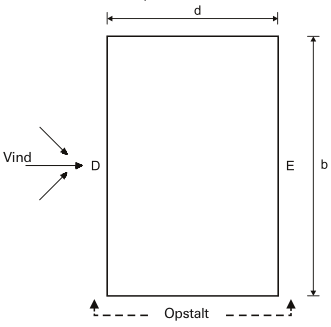
\includegraphics[width=0.9\textwidth]{billeder/vindvest1.png} %Venstre billede
	\end{minipage}\hfill
	\begin{minipage}[b]{0.48\textwidth}\centering
		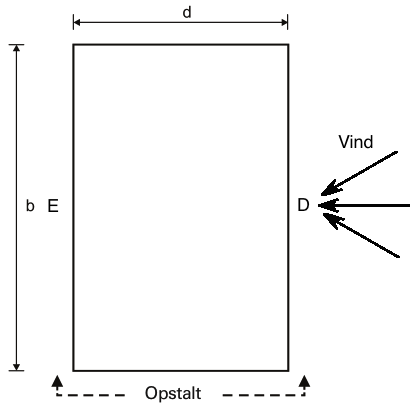
\includegraphics[width=0.9\textwidth]{billeder/vindost1.png} %Højre billede
	\end{minipage}\\ %Captions and labels
	\begin{minipage}[t]{0.48\textwidth}
		\caption{Vind på facaden fra vest \citep[ 7.2.2]{EU91}} %Venstre caption og label
		\label{fig:vindvest}
	\end{minipage}\hfill
	\begin{minipage}[t]{0.48\textwidth}
		\caption{Vind på facaden fra øst \citep[ 7.2.2]{EU91}} %Højre caption og label
		\label{fig:vindost}
	\end{minipage}
\end{figure}

Igen regnes der først en udvendige vindlast på facaderne og derefter en indvendig vindlast på facaderne, inden der opstilles en række vindkombinationer, hvor nettovindtrykket udregnes. For vindkombinationerne ses der bort fra siderne A, B og C, da den midterste ramme ligger 6,25 meter inde i konstruktionen og derfor ikke ligger i zonerne A, B eller C:
\begin{enumerate}
	\item Tryk udvendigt på D og sug indvendigt
	\item Sug udvendigt på E og sug indvendigt
	\item Tryk udvendigt på D og tryk indvendigt  
	\item Sug udvendigt på E og tryk indvendigt
\end{enumerate}

Der arbejdes videre med vindkombination 1, hvor den udvendige vind virker som tryk på siden D og sug på siden E og med en indre vindlast som sug.
\newline \indent{     }  Værdierne for nettovindtrykket kan ses på Figur \ref{tab:hh}.

\begin{table}[htb]
	\begin{center}
		\begin{tabular}{ |c|c|c|c| } 
			\hline
			\multirow{2}{*}{Zone/Formfaktor} & \multirow{2}{*}{$c_{pe,10}$ udvendig} & \multicolumn{2}{l|}{$c_{pe,10}$ indvendig} \\ \cline{3-4} 
			& & Positiv & Negativ   		\\ \hline
			A & -1,200 & 0,200 & -0,300 \\	\hline
			B & -0,800 & 0,200 & -0,300 \\	\hline 
			D & 0,800 & 0,200 & -0,300 \\	\hline
			E & -0,517 & 0,200 & -0,300 \\	\hline
		\end{tabular}
		\caption{Værdier for $c_{pe,10}$ for vind fra vest og øst}
		\label{tab:ff}
	\end{center}
\end{table}

\begin{table}[htb]
	\begin{center}
		\begin{tabular}{ |c|c|c|c| } 
			\hline
			\multirow{2}{*}{Zone/Formfaktor} & \multirow{2}{*}{$c_{pe,10}$ udvendig} & \multicolumn{2}{l|}{$c_{pe,10}$ indvendig} \\ \cline{3-4} 
			& & Positiv & Negativ   		\\ \hline
			A & -1,200 & 0,200 & -0,300 \\	\hline
			B & -0,800 & 0,200 & -0,300 \\	\hline
			C & -0,500 & 0,200 & -0,300 \\	\hline 
			D & 0,752 & 0,200 & -0,300 \\	\hline
			E & -0,404 & 0,200 & -0,300 \\	\hline
		\end{tabular}
		\caption{Værdier for $c_{pe,10}$ for vind fra nord}
		\label{tab:gg}
	\end{center}
\end{table}

\begin{table}[htb]
	\begin{center}
		\begin{tabular}{|c|c|c|c|}
			\hline
			Zone/Vindretning, w $[\frac{kN}{m}]$ & Vest & Øst & Nord \\ \hline
			D & 3,686 & 2,946 & 2,142 \\ \hline
			E & -0,726 & -0,580 & -0,953 \\ \hline
		\end{tabular}
		\caption{Værdier for nettovindtryk på siderne}
		\label{tab:hh}
	\end{center}
\end{table}

Ud fra Tabel \ref{tab:hh} ses det, at værdierne for vest er størst. Det formodes igen, at vindlasten derfor er mere kritisk fra vest end for de to andre vindretninger, og der ses fremover bort fra vinden fra nord og øst. Derfor anvendes lasterne for vest videre i lastkombinationerne, når der skal opstilles lastkombinationer for siden af bygningen.
\newline \indent{     }  Disse linjelaster virker på højden af facaderne, der er siderne D og E, som hver er 16 m høje.
\newline
\newline
\textbf{Opsummering}
\newline
Det er nu bestemt i denne rapport, at der fokuseres på vind fra vest, hvor der optræder forskellige udvendige laster, mens den indre altid optræder som sug. Lasterne er omregnet til linjelaster ved at multiplicere med afstanden mellem rammerne, hvilken er 6,25 m. 
\newline
\newline
Systemet betragtes, hvor der laves beregninger for rammen i midten af konstruktionen, hvilken ligger 6,25 m inde på konstruktionen. Det betyder, rammen ligger mellem zone F og G (se Figur \ref{fig:opdeling}). Derfor udregnes et gennemsnit mellem værdierne for zonerne F og G ved vind på taget, da zonen E for siderne gælder for hele facaden. 
Dog ses det, at værdierne F og G for taget er ens, og dermed er gennemsnitsværdien lig med værdierne for F og G. 
\newline \indent{     }  De vindlaster der virker på det statiske system, som anvendes til videre beregninger, er illustreret på Figur \ref{fig:vindlast}. 

\begin{figure}[htbp]
	\centering
	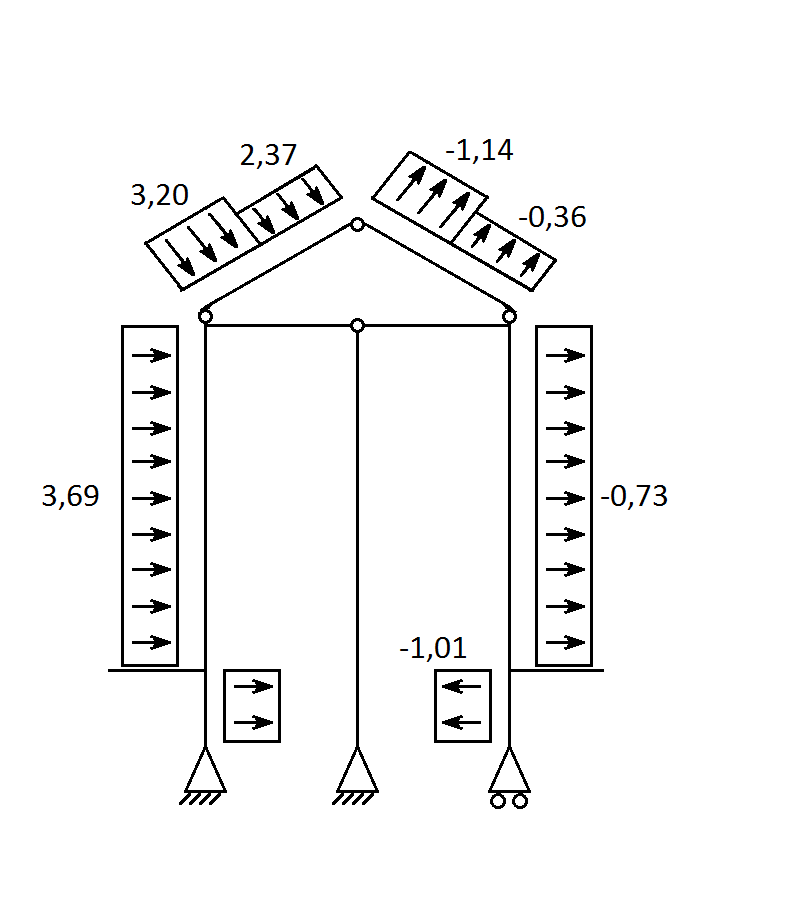
\includegraphics[width=0.5\textwidth]{billeder/vindlast.png}
	\caption{Vindlast på det statiske system angivet i $\frac{kN}{m}$}
	\label{fig:vindlast}
\end{figure}

\subsubsection{Nyttelast}
Ud fra Eurocode 1991 aflæses den jævnt fordelte last, $q_k$, for kategori A1, som er bolig og lokale adgangsveje, til $1,\!5 \frac{kN}{m^2}$ \citep[ tabel 6.2 kapitel 6.3.1.2]{EU91}. Lasten omregnes til en linjelast ved at multiplicere med afstanden mellem rammerne på $6,\!25$ m. Hermed fås en linjelast på $9,\!37 \frac{kN}{m}$. 
\newline \indent{     }  Den nyttelast, der virker på det statiske system er illustreret på Figur \ref{fig:nyttelast}.

\begin{figure}[htbp]
	\centering
	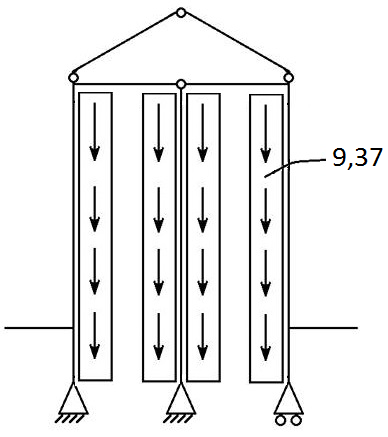
\includegraphics[width=0.4\textwidth]{billeder/nyttelast.png}
	\caption{Nyttelast på det statiske system angivet i $\frac{kN}{m}$}
	\label{fig:nyttelast}
\end{figure}

\section{Lastkombinationer}
Den karakteristiske egenlast, jordlast, vindlast, snelast og nyttelast er bestemt for tilbygningen til Strøybergs Palæ. Derfor opstilles en række lasttilfælde, for at finde de regningsmæssige laster, som skal anvendes til beregningerne af reaktioner. Lastkombinationerne opstilles ved at betragte tilbygningen i de områder, som er illustreret på Figur \ref{fig:omraader}.

\begin{figure}[htbp]
	\centering
	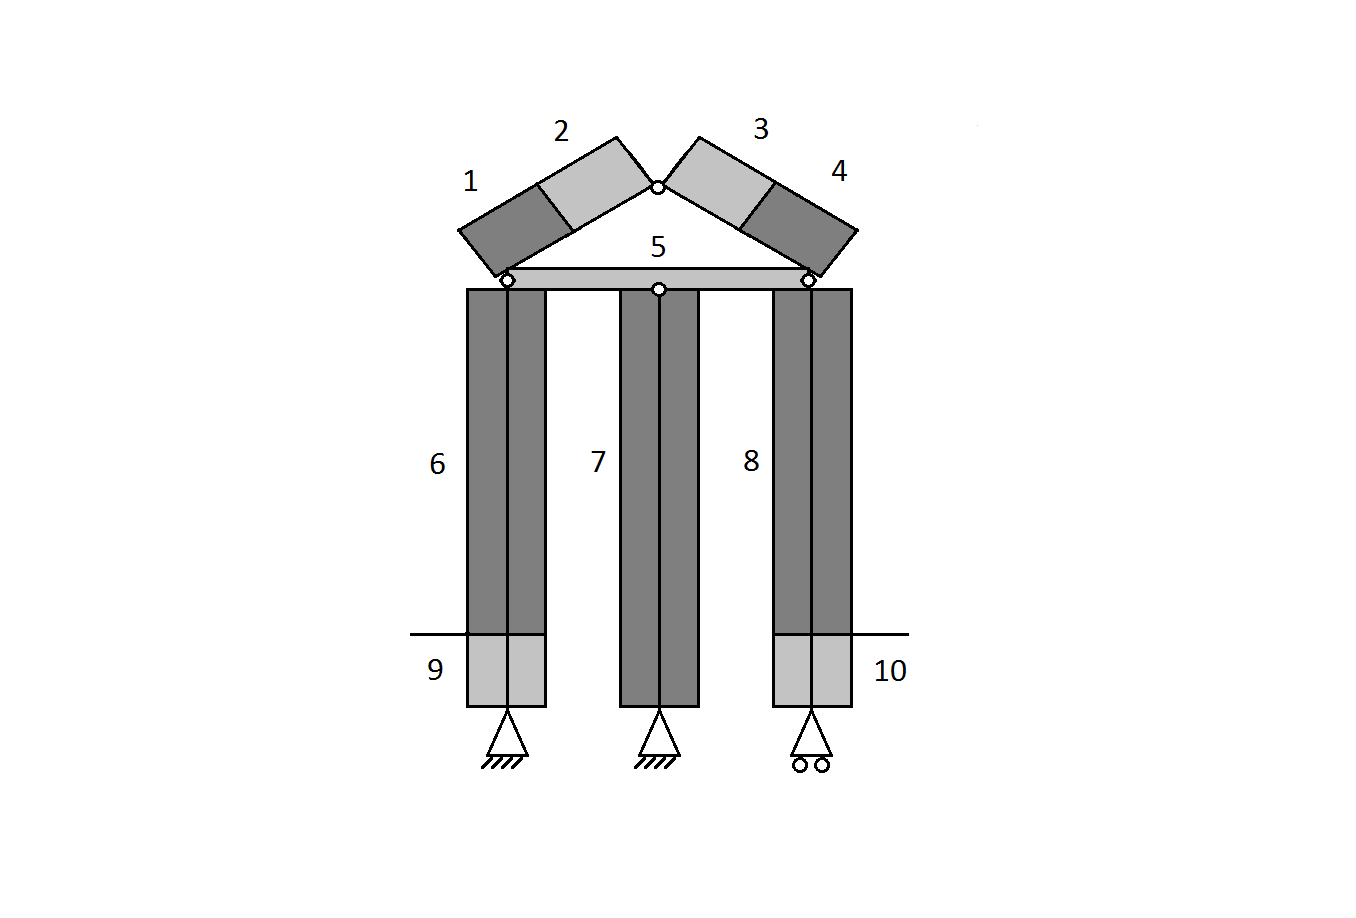
\includegraphics[width=0.3\textwidth]{billeder/indeling.png}
	\caption{Statisk system inddelt i områder}
	\label{fig:omraader}
\end{figure}

Ved et rigtigt byggeprojekt skal der opstilles lasttilfælde for alle tænkelige scenarier, som kan forekomme. For dette projekt er det dog ikke en mulighed, og derfor er der til videre beregninger valgt at fokusere på vindlast som den dominerende last. Hermed opstilles der følgende lastkombination for hvert område:
\begin{center}
	$E_d = \gamma_{G1} K_{FI} G_{K1} + \gamma_{G2} K_{FI} G_{K2} + \gamma_{Q1} K_{FI} Q_{K1} + \gamma_{Q2} \Psi_{0,2} K_{FI} Q_{K2} + \gamma_{Q3} \Psi_{0,3} K_{FI} Q_{K3}$ 
\end{center}

\begin{itemize}
	\item[-] $\gamma_G$: Partialkoefficient for permanent last
	\item[-] $K_{FI}$: Konsekvensklasse
	\item[-] $G_K$: Karakteristisk værdi for permanent last
	\item[-] $\gamma_Q$: Partialkoefficient for variabel last
	\item[-] $Q_K$: Karakteristisk værdi for variabel last
	\item[-] $\Psi$: Kombinationsværdi af variabel last, som mulitipliceres den værdi, som ikke er dominerende 
\end{itemize}

Nedenfor gennemgås to beregningseksempeler for den regningsmæssige last, med udgangspunkt i henholdsvis område 1 og 6. 

I område 1 område optræder der vindlast, snelast og egenlast, og beregnes ved følgende:

\begin{center}
	$E_d = 1,\!0 \cdot 1,\!1 \cdot 8,\!63 \frac{kN}{m} + 1,\!5 \cdot 1,\!1 \cdot 3,\!20 \frac{kN}{m} + 1,\!5 \cdot 0 \cdot 1,\!1 \cdot 5,\!0 \frac{kN}{m}$
\end{center}

Herudfra kan egenlasten, der virker per løbende skrå længde, vindlasten, der virker vinkelret på taget, og snelasten, der virker per løbende vandrette længde, for dette område findes:

\begin{center}
	$Egenlast = 1,\!0 \cdot 1,\!1 \cdot 8,\!63 \frac{kN}{m} = 9,\!49 \frac{kN}{m}$
\end{center}

\begin{center}
	$Vindlast = 1,\!5 \cdot 1,\!1 \cdot 3,\!20 \frac{kN}{m} = 5,\!28 \frac{kN}{m}$
\end{center}

\begin{center}
	$Snelast = 1,\!5 \cdot 0 \cdot 1,\!1 \cdot 5,\!0 \frac{kN}{m} = 0 \frac{kN}{m}$ 
\end{center}

I område 6 optræder der vindlast, egenlast fra etagedæk, egenlast fra stålprofiler og nyttelast. Her er egenlasten for etagedæk og egenlasten fra stålprofilerne lagt sammen til $21,\!64 \frac{kN}{m}$. Lastkombinationen opstilles som følgende:

\begin{center}
	$E_d = 1,\!0 \cdot 1,\!1 \cdot 21,\!64 \frac{kN}{m} + 1,\!5 \cdot 1,\!1 \cdot 3,\!68 \frac{kN}{m} + 1,\!5 \cdot 0,\!5 \cdot 1,\!1 \cdot 9,\!37 \frac{kN}{m}$
\end{center}

De laster der virker i vandret retning, altså i x-retningen, er vindlast:

\begin{center}
	$x-retning = 1,\!5 \cdot 1,\!1 \cdot 3,\!68 \frac{kN}{m} = 6,\!08 \frac{kN}{m}$
\end{center}

De laster der virker i lodret retning, altså y-retningen, er nyttelast, egenlast fra etagedæk samt egenlast fra stålprofiler:

\begin{center}
	$y-retningen = 1,\!0 \cdot 1,\!1 \cdot 21,\!64 \frac{kN}{m} + 1,\!5 \cdot 0,\!5 \cdot 1,\!1 \cdot 9,\!37 \frac{kN}{m} = 31,\!54 \frac{kN}{m}$ 
\end{center}

Ovenstående beregninger gentages hvor hvert område på konstruktionen, og der er derfor lavet i alt 11 lastkombinationer i dette projekt. De laster der virker på konstruktionen er angivet på Figur \ref{fig:laster}. 

\begin{figure}[htbp]
	\centering
	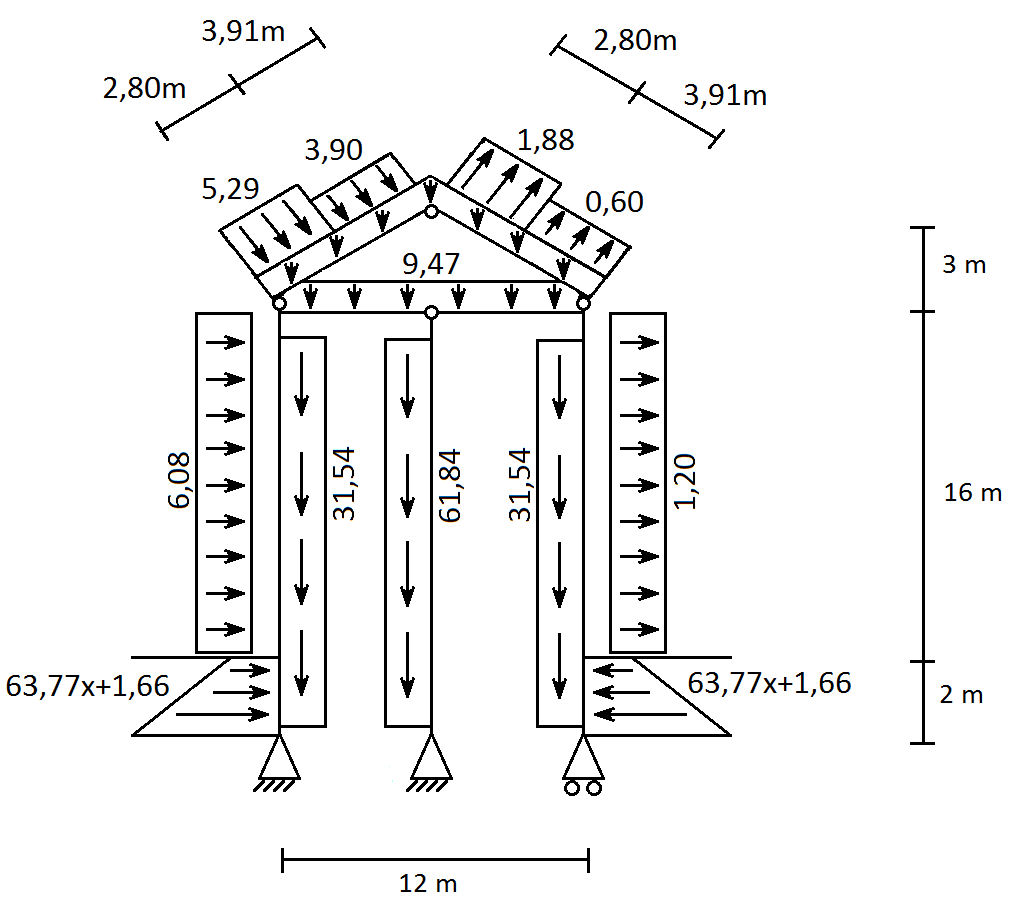
\includegraphics[width=0.7\textwidth]{billeder/vdom.png}
	\caption{Samlede laster på det statiske system med vind fra vest dominerende. Lasterne er angivet i $\frac{kN}{m}$}
	\label{fig:laster}
\end{figure}

Taget i bjælkekonstruktionen er forbundet til den resterende del af konstruktionen via charnierled. Lasterne der virker på taget vil dermed kunne overføres til den resterende del af konstruktionen som punktlaster med angrebspunkt i knudepunkterne, hvor charnierledene er. De reaktioner og laster som virker på taget er illustreret på Figur \ref{fig:tagmedreaktioner}.

\begin{figure}[htbp]
	\centering
	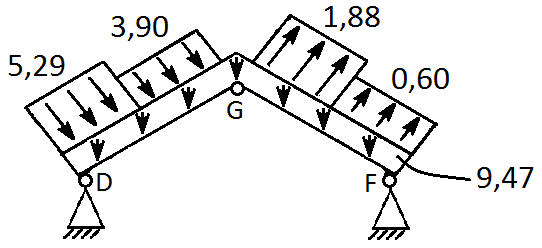
\includegraphics[width=0.7\textwidth]{billeder/tagmedreaktioner.png}
	\caption{Tag med laster og understøtninger. Lasterne er angivet i $\frac{kN}{m}$}
	\label{fig:tagmedreaktioner}
\end{figure}

Punktlasterne bestemmes gennem de tre ligevægtsligninger, ved at beregne reaktionerne i de to punkter, D og F, som begge er fast simple understøttet. Før reaktionerne bestemmes, skal vindlasten, som virker vinkelret på tagoverfladen, deles op i x- og y-komposanter ved at mulitplicere med taghældningen på $26,\!6^\circ$. Egenlasten virker vinkelret på jordoverfladen, og derfor kun i y-retningen. Når vindlasten er opdelt i x- og y-komposanter, samles lasterne for henholdsvis x- og y-retningen. Fritlegemediagrammet samt de laster på taget, som skal bruges til at finde reaktioner, er illustreret på Figur \ref{fig:fld}. 

\begin{figure}[htbp]
	\centering
	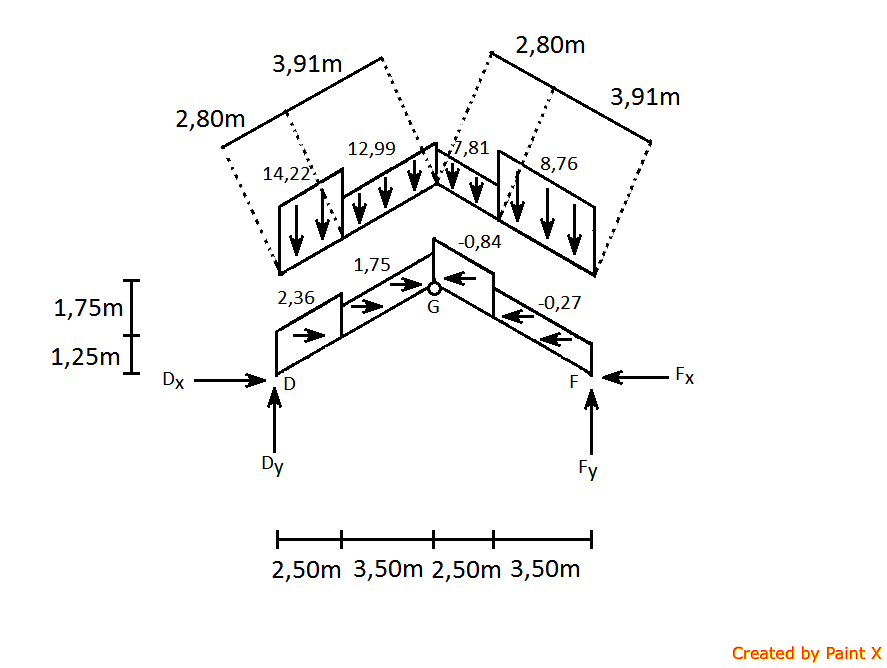
\includegraphics[width=0.7\textwidth]{billeder/fldtag.png}
	\caption{Frilegemediagram. Lasterne er angivet i $\frac{kN}{m}$}
	\label{fig:fld}
\end{figure}

Reaktionerne kan dermed beregnes:
\begin{center}
	Moment om D: $-14,\!221 \frac{kN}{m} \cdot 2,\!795 m \cdot \frac{2,\!5 m}{2} - 12,\!986 \frac{kN}{m} \cdot 3,\!913 m \cdot (2,\!5 m + \frac{3,\!5 m}{2}) - 2,\!364 \frac{kN}{m} \cdot 2,\!795 m \cdot (\frac{1,\!25 m}{2}) - 1,\!746 \frac{kN}{m} \cdot 3,\!913 m \cdot (1,\!25 m + \frac{1,\!75 m}{2}) - 7,\!814 \frac{kN}{m} \cdot 2,\!795 m \cdot (6 m + \frac{2,\!5 m}{2}) - 8,\!960 \frac{kN}{m} \cdot 3,\!913 m \cdot (8,\!5 m + \frac{3,\!5 m}{2}) - (-0,\!840 \frac{kN}{m}) \cdot 2,\!795 m \cdot (1,\!25 m + \frac{1,\!75 m}{2}) - (- 0,\!267 \frac{kN}{m}) \cdot 3,\!913 m \cdot (\frac{1,\!25 m}{2}) + 12 m \cdot f_y = 0 \leftrightarrow f_y = 66,\!366 kN$ 
\end{center}

\begin{center}
	Lodret ligevægt: $-14,\!221 \frac{kN}{m} \cdot 2,\!795 m - 12,\!986 \frac{kN}{m} \cdot 3,\!913 m - 7,\!814 \frac{kN}{m} \cdot 2,\!795 m -  8,\!960 \frac{kN}{m} \cdot 3,\!913 m + d_y + f_y = 0 \leftrightarrow d_y = 81,\!103 kN$
\end{center}

\begin{center}
	Moment om charnier-led (højre del): $- 7,\!814 \frac{kN}{m} \cdot 2,\!795 m \cdot (\frac{2,\!5 m}{2}) - 8,\!960 \frac{kN}{m} \cdot 3,\!913 m \cdot (2,\!5 m + \frac{3,\!5 m}{2}) - (-0,\!840 \frac{kN}{m}) \cdot 2,\!795 m \cdot (\frac{1,\!75 m}{2}) - (- 0,\!267 \frac{kN}{m}) \cdot 3,\!913 m \cdot (1,\!75 m + \frac{1,\!25 m}{2}) + f_y \cdot 6 m - f_x \cdot 3 m = 0 \leftrightarrow f_x = 75,\!474 kN$
\end{center}

\begin{center}
	Vandret ligevægt: $2,\!364 \frac{kN}{m} \cdot 2,\!795 m + 1,\!746 \frac{kN}{m} \cdot 3,\!913 m + 0,\!840 \frac{kN}{m} \cdot 2,\!795 m + 0,\!267 \frac{kN}{m} \cdot 3,\!913 m - f_x + d_x = 0 \leftrightarrow d_x = 58,\!641 kN$
\end{center}

Disse reaktioner virker som punktlast på taget, og det endelige statiske system med de laster der skal bruges til at finde reaktioner for det statiske system, er illustreret på Figur \ref{fig:alle}. 

\begin{figure}[htbp]
	\centering
	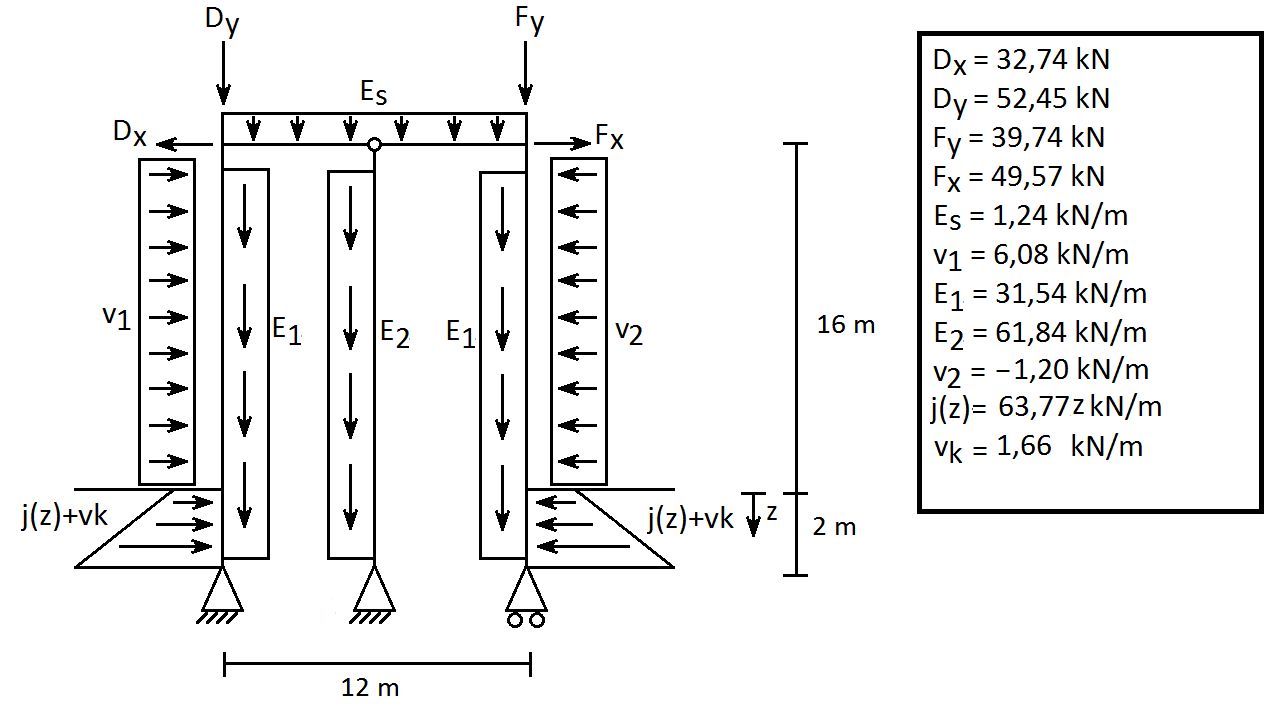
\includegraphics[width=0.7\textwidth]{billeder/endeligesystemmedlaster.png}
	\caption{Statisk system med punktlaster og linjelaster. Linjelasterne er angivet i $\frac{kN}{m}$}
	\label{fig:alle}
\end{figure}
